\documentclass[12pt, a4paper]{article}
\usepackage[UKenglish]{babel}
\usepackage[utf8]{inputenc}
\usepackage{mathtools} % an extension of amsmath
\usepackage{amsthm, amssymb, amsfonts, amstext}
\usepackage{longtable}
\usepackage{tocloft}
\usepackage{geometry}
\usepackage{algpseudocode}
\usepackage{multicol}
\geometry{margin=27mm}
\usepackage{listings}
\usepackage{xcolor,colortbl}
\usepackage{wrapfig}
\usepackage{graphicx}
\usepackage{array}
\usepackage{tabularx}
\usepackage{makecell}
\usepackage{ulem}
% \usepackage[htt]{hyphenat}
% \usepackage{gensymb}
\renewcommand\theadalign{bc} % to leave lines inside a table
\renewcommand\theadgape{\Gape[4pt]}
\renewcommand\cellgape{\Gape[4pt]}
\definecolor{codegreen}{rgb}{0,0.6,0}
\definecolor{codegray}{rgb}{0.5,0.5,0.5}
\definecolor{codepurple}{rgb}{0.58,0,0.82}
\definecolor{backcolour}{rgb}{0,0,0}
\definecolor{pageBG}{rgb}{0,0,0}
\usepackage{hyperref}
\hypersetup{
    colorlinks=true,
    linkcolor=blue,
    filecolor=magenta,
    urlcolor=cyan,
}
\lstdefinestyle{mystyle}{
    backgroundcolor=\color{backcolour},
    commentstyle=\color{yellow},
    keywordstyle=\color{red},
    numberstyle=\color{red},
    stringstyle=\color{codepurple},
    basicstyle=\ttfamily\footnotesize\color{codegreen},
    breakatwhitespace=false,
    breaklines=true,
    captionpos=b,
    keepspaces=true,
    numbers=left,
    numbersep=5pt,
    showspaces=false,
    showstringspaces=false,
    showtabs=false,
    tabsize=4
}
\lstset{style=mystyle}
\urlstyle{same}
\usepackage{cleveref}

\newtheorem{theorem}{Theorem}[section]
\theoremstyle{definition}
\newtheorem{definition}{Definition}[section]
\newtheorem*{claim}{Claim}
\theoremstyle{remark}
\newtheorem*{remark}{Remark}
% \numberwithin{equation}{section}
\newcommand{\textsb}{\textsubscript}

\title{\uwave{Project Surveillance}\\Report}
\author{Aditya Harikrish\\Anusha Nath Roy\\Gaurav Singh\\Yash Anil Bhatia}
\date{}

\begin{document}
\maketitle

\subsection*{Initial Objectives}
Our initial objective was to create a security device that clicked several pictures using an ESP32-Cam module whenever motion was detected by a PIR sensor. The motivation was to save disc space by only clicking pictures when necessary.

\subsection*{Challenges and Consequent Change in Objectives}
We were not able to upload any code to the ESP32-Cam module. We tried several options, but were unable to get it to work. Therefore, we changed our objective while retaining the same theme\textemdash security. We designed
\begin{enumerate}
    \item a radar, and
    \item a motion detection warning system integrated into a Telegram (a popular messaging app) bot for the end user to interact with.
\end{enumerate}

\subsection*{Implementation}
Our circuit is spread across two of our teammates\textemdash Gaurav and Anusha\textemdash due to the constraints of distance learning.

\subsubsection*{Gaurav's End}
Gaurav has the radar. It has a $180^\circ$ sweeping angle. It cycles through 7 angles\textemdash $0^\circ$, $30^\circ$, $60^\circ$, $90^\circ$, $120^\circ$, $150^\circ$ and $180^\circ$\textemdash and records the distance measured by the distance sensor for each of these angles.

Gaurav first runs \texttt{src.py}, which sets up oneM2M by creating a container. On oneM2M, we have 7 graphs that plot distance measured versus time, one for each of the axes along which distance is measured.

Then, he runs \texttt{radar/radar.ino} and \texttt{radar\_plotter.py} simultaneously. \ttfamily radar/\allowbreak radar.ino \normalfont is what runs the radar itself while \texttt{radar\_plotter.py} plots an interactive graph (a spider plot) in \texttt{localhost:8000}, one for each axis (see \cref{fig:RP}).
% Write what this graph measures
% Insert figures of the oneM2M graphs and the radar_plotter.py graph

\begin{figure}[!h]
    \centering
    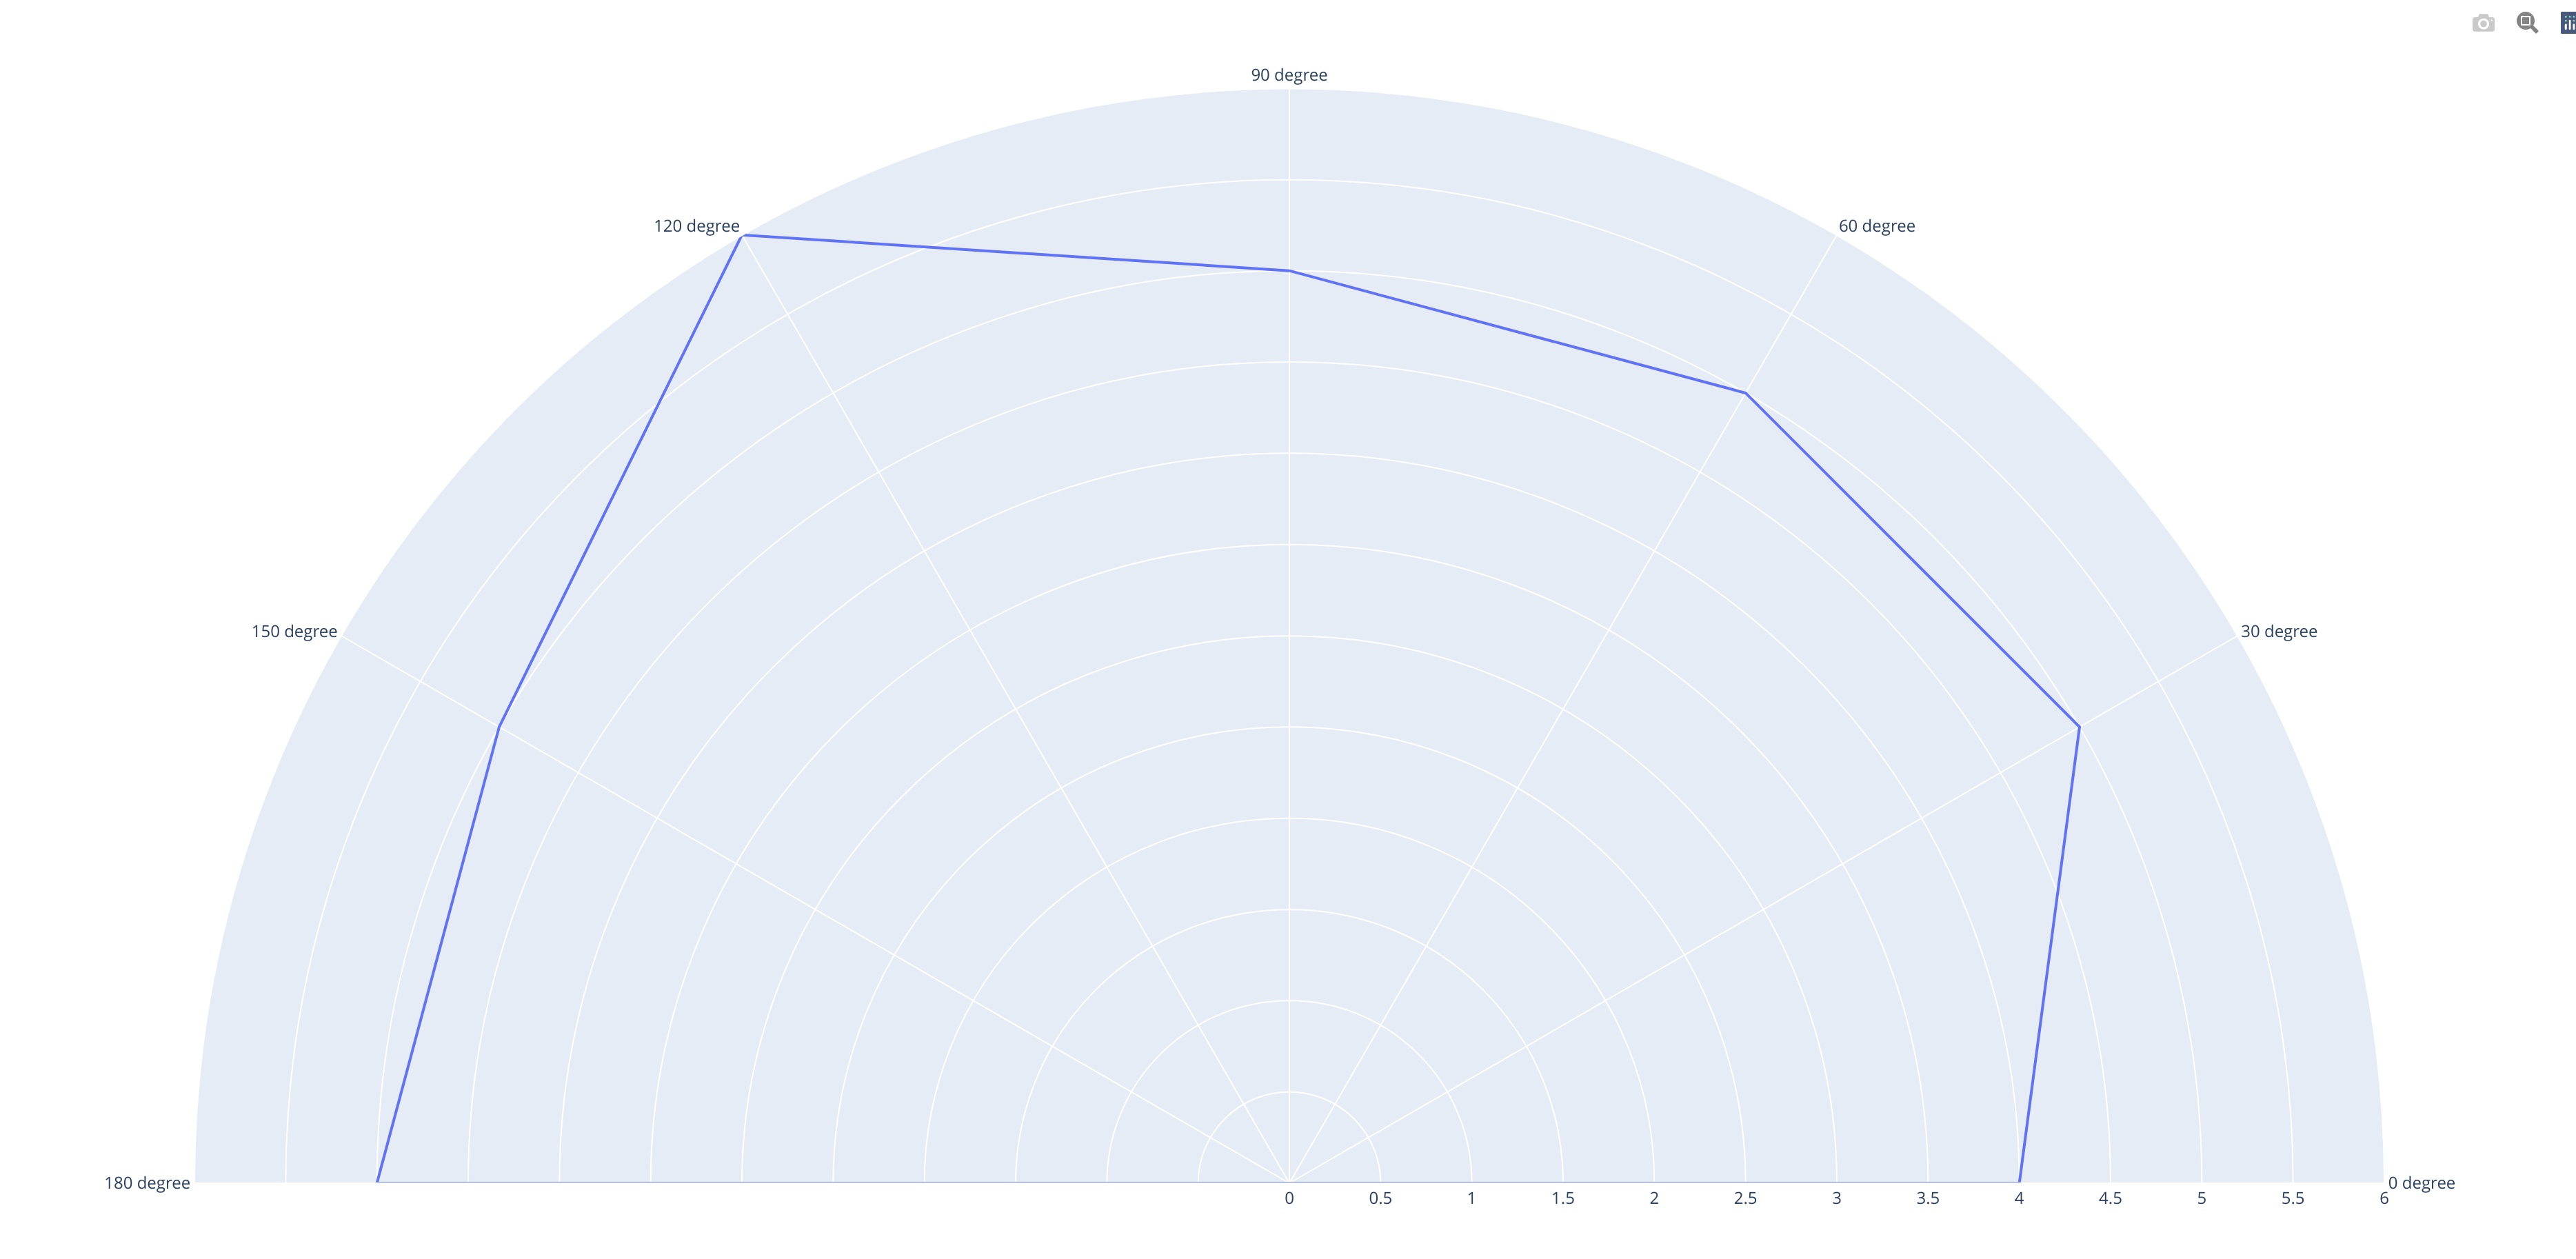
\includegraphics[scale=0.15]{img/RadarPlotter Chart.png}
    \caption{Interactive graph in the browser, plotter by \texttt{radar\_plotter.py}}
    \label{fig:RP}
\end{figure}

\subsubsection*{Anusha's End}
Anusha has the motion detection system. She has a PIR motion sensor along with a buzzer and an LED. Originally, the plan was to integrate both, the radar and the motion sensor into a single system, but that proved infeasible due to online classes. A graph of the number of times motion is detected is plotted on ThingSpeak as a function of time (see \cref{fig:TS}). Anusha runs \texttt{telegram/\allowbreak telegram.ino}, which contains the code for Telegram bot and the end-user's interaction with Anusha's circuit. The bot can be given the following commands:
\begin{enumerate}
    \item \texttt{/start} or \texttt{/help} for a list of commands that can be executed,
    \item \texttt{/led\_warn} to turn the LED on and \texttt{/led\_off} to turn the LED off,
    \item \texttt{/buzzer\_warn} to turn the buzzer on and \texttt{/buzzer\_off} to turn the buzzer off, and
    \item \texttt{/led\_state} and \texttt{/buzzer\_state} to learn about the status of the LED and the buzzer respectively (i.e. whether they are on or off).
\end{enumerate}

\begin{figure}[!t]
    \centering
    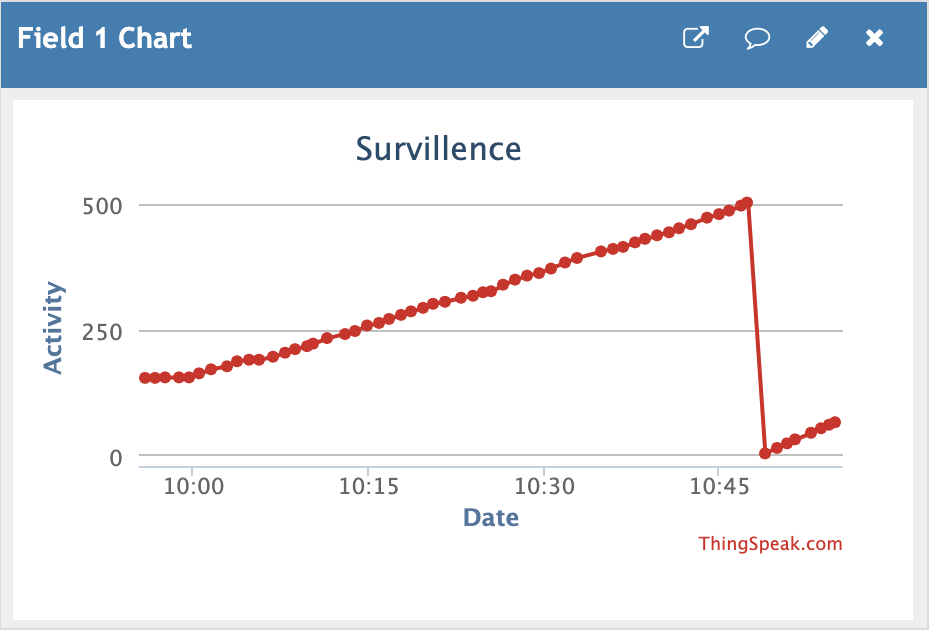
\includegraphics[scale=0.6]{img/ThingSpeak Chart.png}
    \caption{Activity vs time plot on ThingSpeak}
    \label{fig:TS}
\end{figure}


\end{document}

